\section{Architecture}

\subsection{Process view}

This section first introduces the activity diagrams of a few common tasks, and
afterwards goes through the main commands of \pman. The activity
diagrams seek to explain the basic workflow of each command, for example what
is done in event of an error, or when authentication fails etc.

The activity diagrams should act as basis for the implementation of the different
commands, due to the previously mentioned reasons. Clear error handling flow is
critical for the secure usage of \pman.

\subsubsection{Common tasks}

Prompting database password from the command-line and authentication are one of
the more commonly used operations. For this reason, these operations were separated
out from the main commands.

Database password prompt is done whenever, for example, \pman spots that
the login has timed-out, or when the user has not logged in at all while issuing
a command. By default the password prompt must hide the echo from the terminal.
The diagram can be seen in figure \ref{dia:prompt_pw}.

\begin{figure}[H]
    \centering
    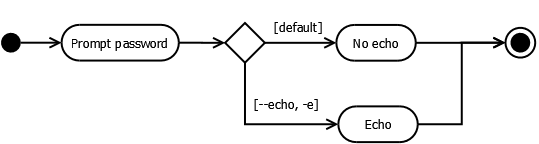
\includegraphics[scale=0.4]{\activitycommon/prompt_pw}
    \caption{Activity diagram for password prompt}
    \label{dia:prompt_pw}
\end{figure}

Much like password prompt, authentication is a very common operation as well.
As \pman allows for saving logins for a set period of time, the
authentication is non-trivial, which is why it is abstracted out of the main
commands. The figure \ref{dia:authenticate} introduces the authentication
workflow.

\begin{figure}[H]
    \centering
    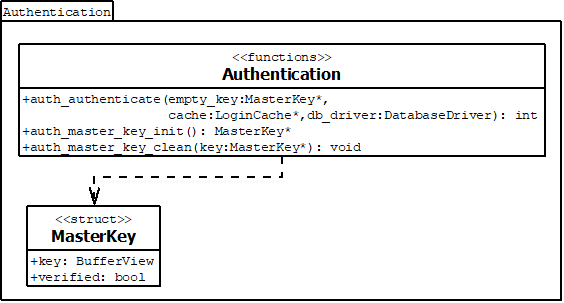
\includegraphics[scale=0.3]{\activitycommon/authenticate}
    \caption{Activity diagram for the authentication process}
    \label{dia:authenticate}
\end{figure}

Accessing the database is something which almost every command does at some
point. The database implements a lot of mechanisms to make breaking into it
that much more difficult, and all of these operations must be abstracted away.

\subsubsection{Main commands}

The main commands are commands that are issued to the \pman in the command line,
which tells the what the user wants to do. Examples of main commands are
initializing a database, adding an entry to database, or listing a database.
These commands form the main workflow of \pman.

The database initialization command \texttt{new} is the very first command
that the user will use with \pman. The activity diagram for this command is
described in figure \ref{dia:init_db}.

\begin{figure}[H]
    \centering
    \centerline{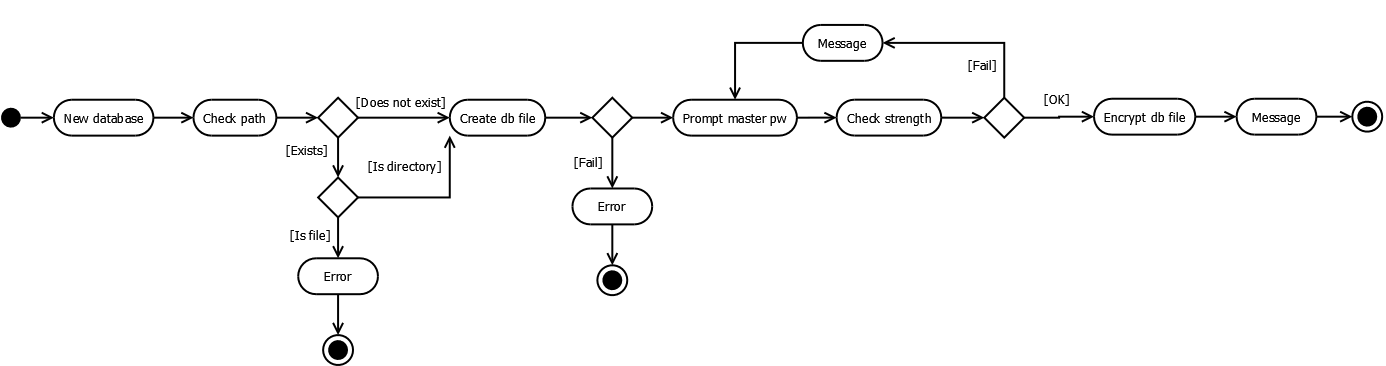
\includegraphics[scale=0.27]{\activitycmds/init_db}}
    \caption{Activity diagram for the database initialization}
    \label{dia:init_db}
\end{figure}

If the initialization of the database is successful, the user will
\texttt{login} to the database either implicitly (by issuing a command), or
explicitly by using the \texttt{login} command. The activity diagram for
\texttt{login} command can be seen in figure \ref{dia:login}.

\begin{figure}[H]
    \centering
    \centerline{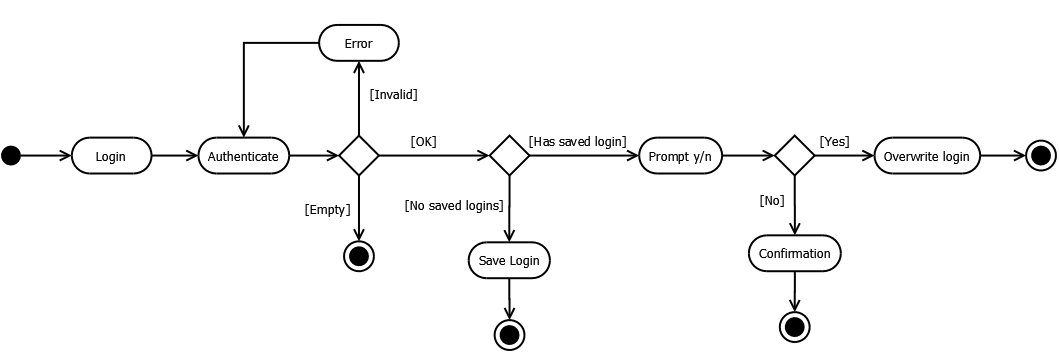
\includegraphics[scale=0.27]{\activitycmds/login}}
    \caption{Activity diagram for logging in to the database}
    \label{dia:login}
\end{figure}

The user can add entries to the database with the \texttt{add} command. The
workflow of this command is described in figure \ref{dia:new_entry}.

\begin{figure}[H]
    \centering
    \centerline{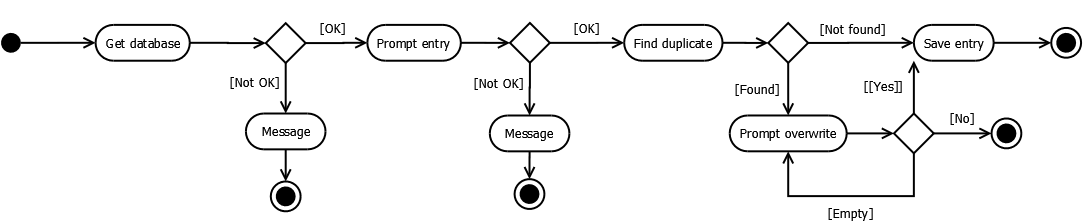
\includegraphics[scale=0.3]{\activitycmds/new_entry}}
    \caption{Activity diagram for adding a new entry}
    \label{dia:new_entry}
\end{figure}

To fetch a password matching a username, the user issues a \texttt{get} command.
The workflow of the \texttt{get} command can be seen in figure \ref{dia:get_pw}.

\begin{figure}[H]
    \centering
    \centerline{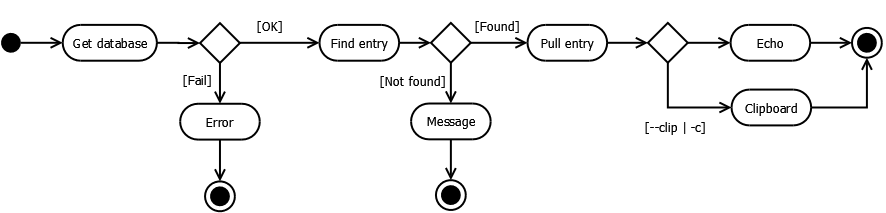
\includegraphics[scale=0.3]{\activitycmds/get_pw}}
    \caption{Activity diagram for fetching a password}
    \label{dia:get_pw}
\end{figure}

Afterwards, the user might want to modify the just added entry in the database.
This can be performed with the \texttt{edit} command and its activity diagram
is visible in figure \ref{dia:edit_entry}.

\begin{figure}[H]
    \centering
    \centerline{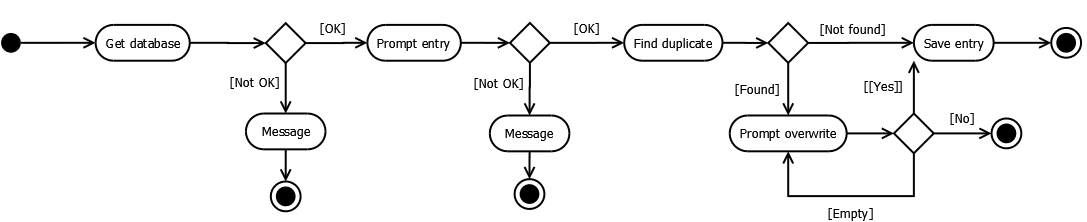
\includegraphics[scale=0.3]{\activitycmds/edit_entry}}
    \caption{Activity diagram for editing an existing entry}
    \label{dia:edit_entry}
\end{figure}

If the user finds that there is an unneeded entry in the database, the user can
issue \texttt{del} command on the entry. This command is described in figure
\ref{dia:delete_entry}.

\begin{figure}[H]
    \centering
    \centerline{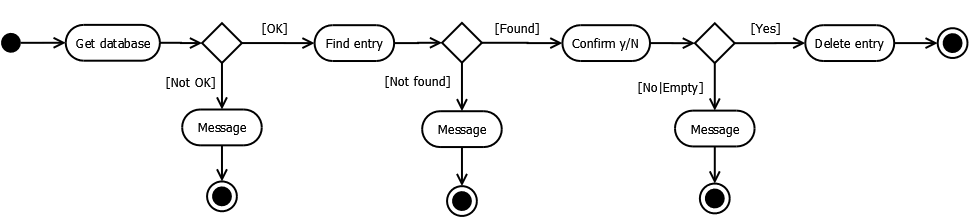
\includegraphics[scale=0.35]{\activitycmds/delete_entry}}
    \caption{Activity diagram for deleting an entry}
    \label{dia:delete_entry}
\end{figure}

Finally, when the user has gathered enough entries in the database, he might
want to view all of the entries. This can be done with the \texttt{list} command,
which is introduced in the figure \ref{dia:list_db}.

\begin{figure}[H]
    \centering
    \centerline{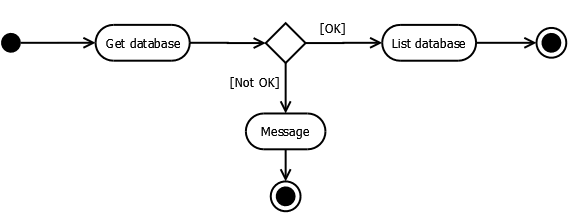
\includegraphics[scale=0.35]{\activitycmds/list_db}}
    \caption{Activity diagram for listing entries in the database}
    \label{dia:list_db}
\end{figure}

The activity diagram for the \texttt{list} command is really simple, as the
implementation details of the command are not a priority.

\subsection{Implementation view}

The main goal of logical view is to present the components of \pman and define
the interface through which they communicate. The primary decisional forces
here are isolating components that require one of the following: emphasis on
security, cross-platform requirements, likely to change over time, or the
component can be generalized to a library.

By making an effort to separate the components of the system this early, we can
minimize the effects of changes to the implementation. That is, as long as the
interfaces are clearly defined. The logical architecture view of \pman is
visible in figure \ref{dia:logical_view}.

\begin{figure}[H]
    \centering
    \centerline{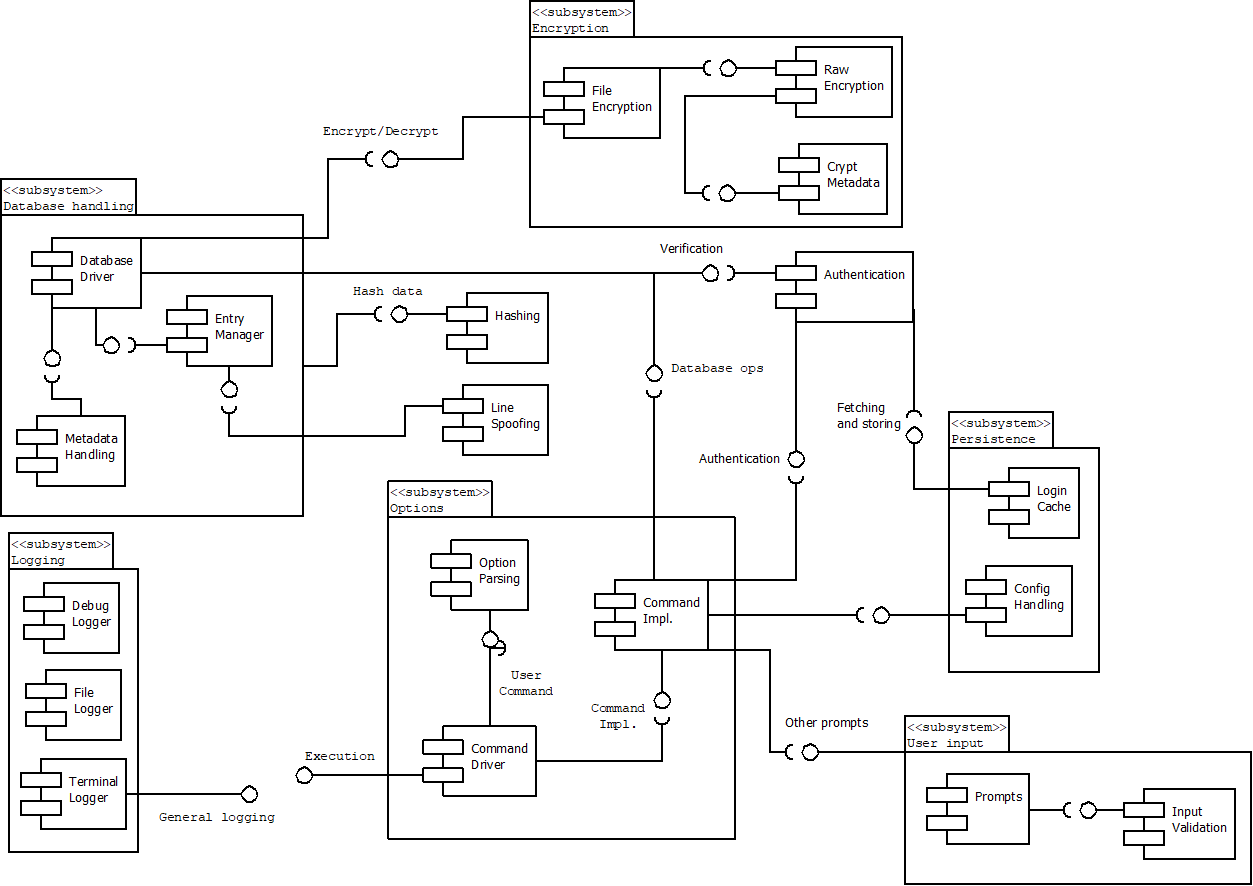
\includegraphics[scale=0.27]{\architectureuml/logical_view}}
    \caption{Logical view of the architecture of \pman}
    \label{dia:logical_view}
\end{figure}

\subsection{Deployment view}

The deployment view seeks to define how \pman is deployed as whole, meaning
what kind of libraries will be built and what will be linked to the executable.
The deployment view also shows the environment the \pman is designed to be
ran in.

The chosen programming language C drives the architectural view quite heavily,
as the entire model of deploying libraries and executables is innate to C. Many
of the libraries linked with \pman are also C libraries. The deployment view
can be seen in figure \ref{dia:deployment_view}.

\begin{figure}[H]
    \centering
    \centerline{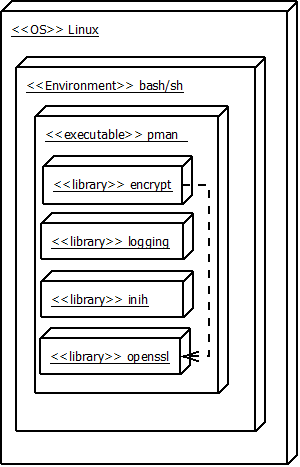
\includegraphics[scale=0.7]{\architectureuml/deployment_view}}
    \caption{Deployment view of the architecture of \pman}
    \label{dia:deployment_view}
\end{figure}

As is apparent in figure \ref{dia:deployment_view}, the execution environment
is almost solely consist of terminal utilities innate to Linux. Other than that,
the \pman executable is linked with cryptographic utilities like \texttt{openssl}
and configuration file libraries \texttt{inih}. The build process also produces
its own libraries like \texttt{logging} and \texttt{encrypt}.
